\section{A Taxonomy of Compression Techniques for Deep Stereo}
\label{sec:taxonomy}

This section is the technical core of the survey. We organize the compression literature into seven families. Fig.~\ref{fig:taxonomy} summarizes the families visually; Table~\ref{tab:compression_families} lists representative methods, the cost axis each family attacks, the mechanism, and the typical effect on cross-domain generalization. Sections~\ref{ssec:backbone}--\ref{ssec:nas} discuss each family in turn.

\begin{figure*}[!htbp]
\centering
% Taxonomy of compression techniques drawn in TikZ.
% 4 columns on top row, 3 columns on bottom row.
\definecolor{famBlue}{RGB}{31,119,180}
\definecolor{famGreen}{RGB}{44,160,44}
\definecolor{famRed}{RGB}{214,39,40}
\definecolor{famPurple}{RGB}{148,103,189}
\definecolor{famOrange}{RGB}{255,127,14}
\definecolor{famBrown}{RGB}{140,86,75}
\definecolor{famTeal}{RGB}{23,190,207}

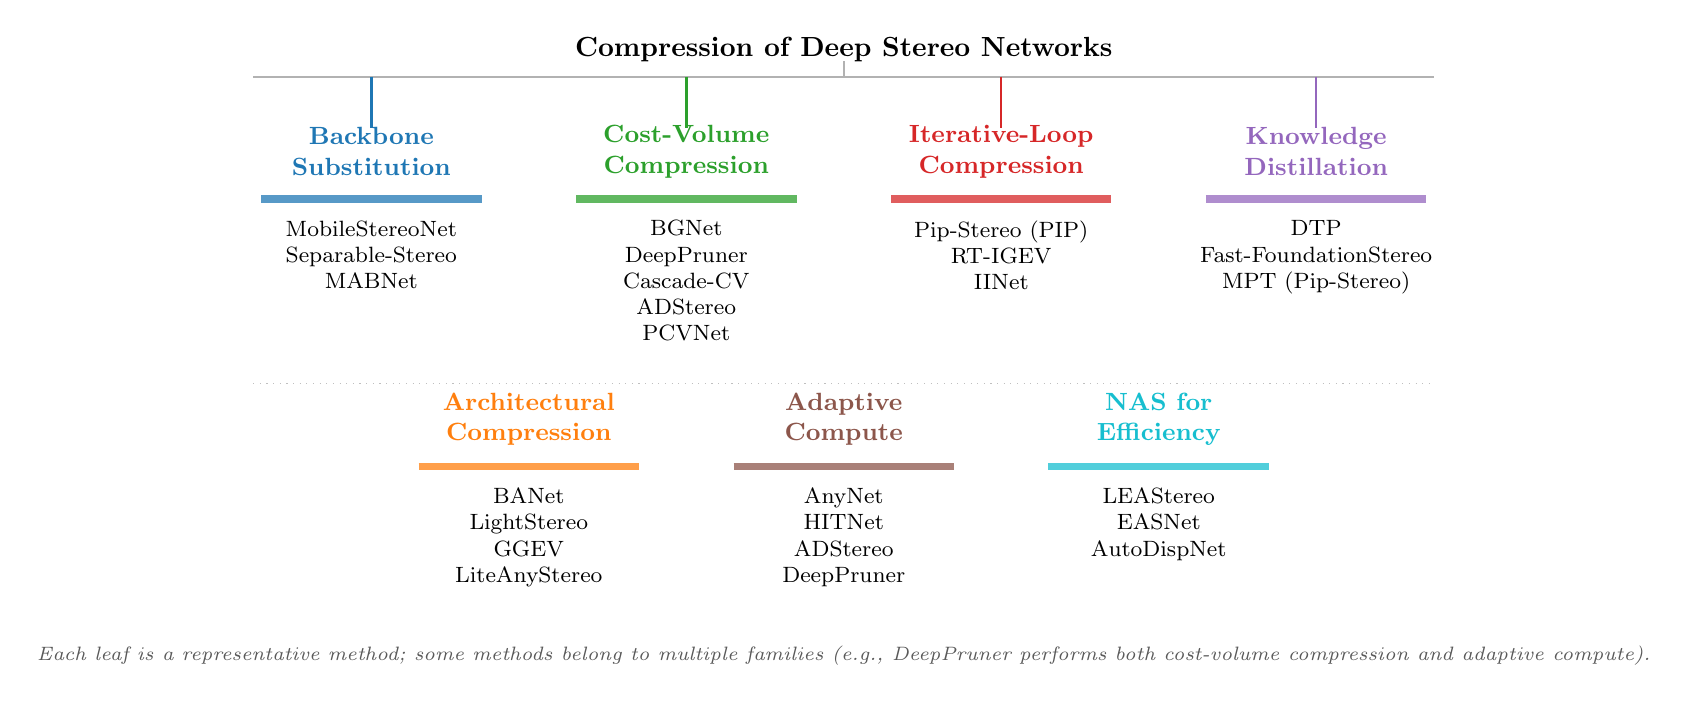
\begin{tikzpicture}[
  every node/.style = {font=\small},
  root/.style = {font=\bfseries},
  branch/.style = {line width=0.9pt, draw=gray!60},
  famheader/.style = {font=\bfseries\small, align=center,
                      text width=3.4cm, inner sep=2pt},
  rail/.style = {line width=2.8pt, draw opacity=0.75},
  methodlist/.style = {font=\footnotesize, align=center,
                       text width=3.2cm, inner sep=2pt}
]

% --- Root and trunk ---
\node[root] (root) at (0, 6.2) {Compression of Deep Stereo Networks};
\draw[branch] (-7.5, 5.85) -- (7.5, 5.85);
\draw[branch] (0, 6.05) -- (0, 5.85);

% ================= TOP ROW =================
% Backbone Substitution
\draw[branch, draw=famBlue] (-6.0, 5.85) -- (-6.0, 5.2);
\node[famheader, text=famBlue] at (-6.0, 4.9) {Backbone\\Substitution};
\draw[rail, draw=famBlue] (-7.4, 4.3) -- (-4.6, 4.3);
\node[methodlist, anchor=north] at (-6.0, 4.1)
  {MobileStereoNet \\ Separable-Stereo \\ MABNet};

% Cost-Volume Compression
\draw[branch, draw=famGreen] (-2.0, 5.85) -- (-2.0, 5.2);
\node[famheader, text=famGreen] at (-2.0, 4.9) {Cost-Volume\\Compression};
\draw[rail, draw=famGreen] (-3.4, 4.3) -- (-0.6, 4.3);
\node[methodlist, anchor=north] at (-2.0, 4.1)
  {BGNet \\ DeepPruner \\ Cascade-CV \\ ADStereo \\ PCVNet};

% Iterative-Loop Compression
\draw[branch, draw=famRed] (2.0, 5.85) -- (2.0, 5.2);
\node[famheader, text=famRed] at (2.0, 4.9) {Iterative-Loop\\Compression};
\draw[rail, draw=famRed] (0.6, 4.3) -- (3.4, 4.3);
\node[methodlist, anchor=north] at (2.0, 4.1)
  {Pip-Stereo (PIP) \\ RT-IGEV \\ IINet};

% Knowledge Distillation
\draw[branch, draw=famPurple] (6.0, 5.85) -- (6.0, 5.2);
\node[famheader, text=famPurple] at (6.0, 4.9) {Knowledge\\Distillation};
\draw[rail, draw=famPurple] (4.6, 4.3) -- (7.4, 4.3);
\node[methodlist, anchor=north] at (6.0, 4.1)
  {DTP \\ Fast-FoundationStereo \\ MPT (Pip-Stereo)};

% --- Divider between rows ---
\draw[dotted, gray!50] (-7.5, 1.95) -- (7.5, 1.95);

% ================= BOTTOM ROW =================
% Architectural Compression
\node[famheader, text=famOrange] at (-4.0, 1.5) {Architectural\\Compression};
\draw[rail, draw=famOrange] (-5.4, 0.9) -- (-2.6, 0.9);
\node[methodlist, anchor=north] at (-4.0, 0.7)
  {BANet \\ LightStereo \\ GGEV \\ LiteAnyStereo};

% Adaptive Compute
\node[famheader, text=famBrown] at (0, 1.5) {Adaptive\\Compute};
\draw[rail, draw=famBrown] (-1.4, 0.9) -- (1.4, 0.9);
\node[methodlist, anchor=north] at (0, 0.7)
  {AnyNet \\ HITNet \\ ADStereo \\ DeepPruner};

% NAS for Efficiency
\node[famheader, text=famTeal] at (4.0, 1.5) {NAS for\\Efficiency};
\draw[rail, draw=famTeal] (2.6, 0.9) -- (5.4, 0.9);
\node[methodlist, anchor=north] at (4.0, 0.7)
  {LEAStereo \\ EASNet \\ AutoDispNet};

% Footer
\node[align=center, font=\scriptsize\itshape, text=gray!70!black]
  at (0, -1.5) {Each leaf is a representative method; some methods belong to multiple families (e.g., DeepPruner performs both cost-volume compression and adaptive compute).};

\end{tikzpicture}

\caption{Taxonomy of compression techniques for deep stereo matching. Seven families are identified; representative methods are listed at the leaves. Many methods belong to multiple families simultaneously: for example, Pip-Stereo~\cite{zheng2026pipstereo} performs both iterative-loop compression and knowledge distillation, and DTP~\cite{pan2024dtp} performs distillation followed by structural pruning.}
\label{fig:taxonomy}
\end{figure*}

% Table summarizing the seven compression families surveyed.
\begin{table*}[!htbp]
\centering
\caption{The seven compression families surveyed in this paper, with representative methods, the cost-axis they primarily reduce, and their typical effect on cross-domain generalization.}
\label{tab:compression_families}
\renewcommand{\arraystretch}{1.15}
\footnotesize
\begin{tabular}{p{2.6cm}p{4.0cm}p{2.4cm}p{4.0cm}p{2.6cm}}
\toprule
\textbf{Family} & \textbf{Representative methods} & \textbf{Cost axis attacked} & \textbf{Mechanism (one sentence)} & \textbf{Typical generalization effect} \\
\midrule
Backbone substitution &
MobileStereoNet~\cite{shamsafar2022mobilestereonet}, Separable-Stereo~\cite{rahim2021separable}, MABNet~\cite{xing2020mabnet} &
Feature extractor FLOPs &
Replace ResNet/UNet with MobileNet-style depthwise-separable backbones. &
Mild loss; recoverable with HVT augmentation. \\
\midrule
Cost-volume compression &
BGNet~\cite{xu2021bgnet}, DeepPruner~\cite{duggal2019deeppruner}, Cascade-CV~\cite{gu2020cascade}, ADStereo~\cite{wang2023adstereo}, PCVNet~\cite{zeng2023pcvnet} &
3D-volume memory \& 3D-conv FLOPs &
Build the cost volume at lower resolution, then refine; or prune unlikely disparity hypotheses. &
Generally preserved; pruning can hurt thin structures. \\
\midrule
Iterative-loop compression &
Pip-Stereo~\cite{zheng2026pipstereo}, RT-IGEV (variant of \cite{xu2023igev}), IINet~\cite{li2024iinet} &
GRU iteration count &
Compress an $r$-fold composition of the GRU update operator into a single learned operator. &
Strong; iteration retains cross-domain robustness. \\
\midrule
Knowledge distillation &
DTP~\cite{pan2024dtp}, Fast-FoundationStereo~\cite{wen2026fastfoundationstereo}, MPT (Pip)~\cite{zheng2026pipstereo} &
Backbone size \& foundation prior &
Distill foundation-model features into a compact student trained with feature-matching losses. &
Strong if teacher is foundation-quality. \\
\midrule
Architectural compression &
BANet~\cite{xu2025banet}, LightStereo~\cite{guo2025lightstereo}, GGEV~\cite{liu2026ggev}, LiteAnyStereo~\cite{jing2025liteanystereo} &
Both feature \& cost-volume FLOPs &
Hand-designed lightweight blocks (bilateral aggregation, channel-boost MLP, etc.) replacing 3D-conv hourglasses. &
Variable; depends on training-data mix. \\
\midrule
Adaptive compute &
AnyNet~\cite{wang2019anynet}, HITNet~\cite{tankovich2021hitnet}, ADStereo~\cite{wang2023adstereo}, DeepPruner~\cite{duggal2019deeppruner} &
Per-region compute &
Spend more compute on high-uncertainty regions and less on confident, textured regions. &
Mostly preserved; learns where to look. \\
\midrule
Neural architecture search &
LEAStereo, EASNet, AutoDispNet~\cite{saikia2019autodispnet} &
Architectural overhead per FLOP &
Search the architecture (cells, operations, topology) to maximize accuracy at fixed compute. &
Limited generalization beyond search domain. \\
\bottomrule
\end{tabular}
\end{table*}


\subsection{Backbone Substitution}
\label{ssec:backbone}

The simplest form of compression is to replace the feature-extraction backbone with a smaller alternative. The standard choice in pre-2020 stereo work was a ResNet-50 or modified UNet, contributing 5--10\,M parameters and a substantial fraction of the inference time. The mobile-vision community produced two natural replacements (depthwise-separable MobileNet variants~\cite{shamsafar2022mobilestereonet} and the more recent EfficientViT family), both of which trade representational capacity for FLOPs.

\textbf{MobileStereoNet}~\cite{shamsafar2022mobilestereonet} is the canonical example: it ports the PSMNet~\cite{chang2018psmnet} 3D-cost-volume design to a MobileNetV2 backbone, producing a $\sim$2.4\,M-parameter network at the cost of $\sim$0.7\% additional KITTI D1 error. \textbf{Separable-Stereo}~\cite{rahim2021separable} extends this idea to the 3D-convolutional regularizer: it replaces full 3D convolutions with depthwise-separable factorizations $(D \times H \times W) \to (D \times 1 \times 1) \times (1 \times H \times W)$, reducing 3D-conv FLOPs by roughly $1/k$ for a $k \times k \times k$ kernel. \textbf{MABNet}~\cite{xing2020mabnet} introduces multi-branch adjustable bottleneck blocks that allow accuracy/efficiency tuning post-training by selecting which branch is active.

The trade-off is well understood: a smaller backbone produces less expressive features, and the cost-volume regularizer must compensate. Empirically, accuracy on the source-domain benchmark (KITTI 2015) typically degrades by $\sim$0.5--1.0\% D1, while latency drops by 2--5$\times$. The cross-domain generalization penalty is typically modest, particularly when training augmentation (HVT~\cite{chang2023hvt}) is applied; we discuss this in Section~\ref{sec:generalization}.

\subsection{Cost-Volume Compression}
\label{ssec:costvol}

The cost volume is the most expensive single tensor in nearly every stereo network: at quarter resolution and a maximum disparity of 192, a concatenation cost volume contains $192 \times H/4 \times W/4 \times 2C$ floats, easily exceeding 1\,GB at typical resolutions. Three families of compression target this tensor.

\subsubsection{Resolution Pyramid (Cascade)}

The first technique builds the cost volume at a low resolution, then refines a narrower disparity range at progressively higher resolutions. Cascade Cost Volume~\cite{gu2020cascade} formalizes this for both stereo and multi-view stereo. At stage $k$, the disparity hypothesis range is
\begin{equation}
R_{k+1} \;=\; R_k \cdot w_k, \qquad I_{k+1} \;=\; I_k \cdot p_k
\label{eq:cascade}
\end{equation}
where $R_k$ is the disparity-range width at stage $k$, $I_k$ is the disparity sampling interval (resolution), $w_k \in (0, 1]$ is a learned narrowing factor, and $p_k$ is a refinement factor. Each cost volume has a fixed $D \approx 48$ disparity bins regardless of stage; after $K = 3$ stages, the system has covered the full $192$-disparity range while only ever materializing a 48-bin volume. Empirically, this reduces 3D-conv FLOPs by 30--50$\times$ relative to a single-stage volume at the same final resolution. CFNet~\cite{shen2021cfnet} extends Cascade Cost Volume with cross-stage feature fusion; ACVNet~\cite{xu2022acvnet} replaces the cascade with an attention-based confidence weighting that achieves a similar effect.

\subsubsection{Bilateral Grid (BGNet)}

A complementary technique is to construct the cost volume in a low-dimensional bilateral grid rather than a full 4D tensor. BGNet~\cite{xu2021bgnet} stores the cost volume in a grid indexed by spatial coordinates and image intensity (rather than by every pixel and disparity); the slicing operation that recovers a per-pixel disparity is fast because the grid is smaller and respects edges in the input image. The result is a $2$--$5\times$ memory reduction with minimal accuracy loss.

\subsubsection{Pruning the Disparity Hypothesis Set (DeepPruner)}

A third technique is to prune disparity hypotheses that are unlikely. DeepPruner~\cite{duggal2019deeppruner} uses a differentiable PatchMatch step to estimate, for each pixel, a small number of candidate disparities; the cost volume is then evaluated only at these candidates. This can reduce cost-volume compute by an order of magnitude for scenes with low disparity entropy, but at the price of catastrophic failure on high-uncertainty pixels (transparent surfaces, occlusions) where the candidate set is poorly chosen. ADStereo~\cite{wang2023adstereo} pursues an analogous content-aware downsampling that adapts the spatial resolution of the cost volume rather than the disparity range.

\subsubsection{Parameterized Cost Volume (PCVNet)}

PCVNet~\cite{zeng2023pcvnet} parameterizes the cost volume as a Gaussian mixture rather than as a discrete tensor of similarity scores. The parameters of the mixture (mean, variance, weight per component) are predicted by a small head; the cost volume is reconstructed on-the-fly only at the disparities being queried. The effect is a 4--10$\times$ memory reduction at the cost of increased FLOPs per query, which is a favorable trade on memory-bound edge accelerators.

\subsection{Iterative-Loop Compression}
\label{ssec:iterloop}

The iterative-refinement paradigm (Section~\ref{sec:background}) trades depth for time: rather than apply a single deep regularizer, iterative methods apply a shallow GRU operator $T$ times. The headline accuracy of IGEV-Stereo~\cite{xu2023igev} and IGEV++~\cite{xu2025igevpp} is achieved at $T = 32$ iterations; reducing $T$ naively (the obvious efficiency lever) causes catastrophic accuracy degradation. \textbf{RT-IGEV} (the real-time variant in~\cite{xu2023igev}) drops $T$ to $6$ and reports an EPE increase of about 6\% on Scene Flow, which is the best previously documented direct truncation result.

\textbf{Pip-Stereo}~\cite{zheng2026pipstereo} introduces \emph{Progressive Iteration Pruning} (PIP), which addresses the truncation problem by training a sequence of models in which each successive model approximates an $r$-fold composition of the previous model's GRU operator. Concretely, let $F_\theta : \mathbb{R}^d \to \mathbb{R}^d$ be the trained ConvGRU update operator of a teacher running for $T$ iterations, with hidden states $z_t^{\mathrm{Mi}} \in \mathbb{R}^d$ evolving as
\begin{equation}
z_{t+1}^{\mathrm{Mi}} = F_\theta\!\left(z_t^{\mathrm{Mi}}\right),
\label{eq:mi_rnn}
\end{equation}
for $t = 0, \ldots, T-1$. PIP trains a student operator $G_\phi$ running for $S = T/r$ iterations:
\begin{equation}
z_{s+1}^{\mathrm{Fi}} = G_\phi\!\left(z_s^{\mathrm{Fi}}\right),
\label{eq:fi_rnn}
\end{equation}
for $s = 0, \ldots, S-1$, with the constraint that $G_\phi$ should approximate the $r$-fold composition of $F_\theta$. Training is supervised by aggregating the teacher's intermediate disparities into blocks of size $r$:
\begin{equation}
\bar{d}_s^{\mathrm{Mi}} \;=\; \frac{1}{r} \sum_{i=1}^{r} \Psi\!\left(z_{r(s-1)+i}^{\mathrm{Mi}}\right),
\label{eq:agg}
\end{equation}
for $s = 1, \ldots, S$, where $\Psi$ is the disparity head. The student is trained to match the block-aggregated teacher signal at every iteration:
\begin{equation}
\mathcal{L}_{\mathrm{PIP}} \;=\; \sum_{s=1}^{S} \bigl\Vert \Psi\!\left(z_s^{\mathrm{Fi}}\right) - \bar{d}_s^{\mathrm{Mi}} \bigr\Vert_1 .
\label{eq:pip_loss}
\end{equation}
Pip-Stereo applies PIP recursively, halving $T$ at each step ($32 \to 16 \to 8 \to 4 \to 2 \to 1$). The reported result is striking: at $T = 1$ iteration, Pip-Stereo achieves Scene Flow EPE 0.45, better than the original IGEV-Stereo at $T = 12$ iterations and 11.5$\times$ faster than DEFOM-Stereo on a Jetson Orin NX~\cite{zheng2026pipstereo}.

The conceptual contribution of PIP is the realization that iterative refinement is wasteful in a specific sense: by iteration~32 of an IGEV update, fewer than 1\% of pixels are still being meaningfully updated~\cite{zheng2026pipstereo}, but the GRU is still being run on every pixel. PIP compresses the temporal redundancy without altering the spatial structure of the network.

\subsection{Knowledge Distillation}
\label{ssec:distill}

Distillation in stereo predates the foundation-model era. HITNet~\cite{tankovich2021hitnet}, for instance, uses intra-network distillation between tile-based predictions and a final disparity head. Distillation has become substantially more important since 2024, however, because the foundation methods provide an excellent teacher.

\textbf{Distill-then-Prune (DTP)}~\cite{pan2024dtp} formalizes a two-stage pipeline: (i) distill an IGEV-Stereo teacher's per-iteration cost-volume features into a smaller student that uses fewer 3D-conv channels; (ii) apply a structural pruning step to the student that removes individual cost-volume channels found to contribute negligibly. The reported result is DTP-IGEV-S2 at 1.90\% KITTI D1 and 24~ms latency on RTX 3090, only $\sim$0.3\% worse than IGEV-Stereo at 8$\times$ the speed.

\textbf{Fast-FoundationStereo}~\cite{wen2026fastfoundationstereo} performs cross-architecture distillation: a FoundationStereo teacher (with a Depth Anything V2 ViT backbone) supervises an EfficientViT-based student. The student inherits the foundation prior through feature-matching losses at multiple resolutions but never runs the heavy ViT at inference. The reported result is 1.74\% KITTI D1 at 85~ms on RTX 4090, the best foundation-derived efficient model at the time of writing.

\textbf{Pip-Stereo's MPT}~\cite{zheng2026pipstereo} (Monocular Prior Transfer) is a similar idea applied to the iterative paradigm: the Depth Anything V2 ViT teacher supervises a NAS-searched RepViT student via a multi-resolution feature-alignment loss, and the teacher is discarded at inference. The MPT student carries the monocular knowledge in its weights without any ViT computation at inference time.

The empirical pattern across all three is consistent: a foundation teacher transfers cross-domain robustness to a much smaller student, but only when the student is large enough to absorb the teacher's representational capacity (typically 4--12\,M parameters; smaller students plateau).

\subsection{Architectural Compression}
\label{ssec:arch}

A fifth family makes no use of distillation and no use of cascading; it simply hand-designs a more efficient architecture. The 2024--2026 wave of architectural compression has produced four notable variants.

\textbf{BANet}~\cite{xu2025banet} replaces the standard 3D-convolutional hourglass with a Bilateral Aggregation Network: a 2D context branch and a 3D matching branch fuse via a bilateral grid (in spirit similar to BGNet, but applied to the entire regularizer rather than just the cost volume). At its mobile setting BANet reports 1.4\,M parameters and 12~ms on RTX 3090 at 2.30\% KITTI D1, the fastest model in our comparison among non-iterative architectures.

\textbf{LightStereo}~\cite{guo2025lightstereo} pursues an extreme position: it eliminates the 3D-convolutional regularizer altogether, replacing it with a 2D-only ``channel boost MLP'' that operates on a flattened cost volume. At its largest setting (LightStereo-L) it achieves 1.94\% KITTI D1 at 40~ms, demonstrating that 3D convolutions are not architecturally necessary for high-accuracy stereo.

\textbf{GGEV}~\cite{liu2026ggev} (Geometry-Guided Encoding Volume) uses a geometry-aware feature aggregator that incorporates explicit epipolar-line context. The result is a 2.5\,M-parameter network at 18~ms with 2.20\% KITTI D1.

\textbf{LiteAnyStereo}~\cite{jing2025liteanystereo} packages a foundation-aware compact architecture into a single-shot inference path, reporting 1.97\% KITTI D1 at 30~ms with 4.6\,M parameters. It is, alongside Pip-Stereo and DTP, among the strongest 2025 efficient models on cross-domain benchmarks.

\subsection{Adaptive Compute}
\label{ssec:adaptive}

The sixth family spends compute non-uniformly across the spatial extent of the input, on the principle that easy regions (textured, well-lit, fronto-parallel surfaces) need little processing while hard regions (occlusion boundaries, transparent surfaces, large-depth-discontinuity edges) need more.

\textbf{AnyNet}~\cite{wang2019anynet} is the canonical example of \emph{anytime inference}: the network runs in stages of increasing accuracy and can be terminated at any stage to produce a usable disparity map. The four stages of AnyNet correspond to different latency/accuracy trade-offs (12--40\,ms on Jetson TX2, with KITTI D1 ranging from 6.2\% at the earliest stage to roughly 4\% at the deepest), and the runtime can choose adaptively based on a budget signal. \textbf{HITNet}~\cite{tankovich2021hitnet} performs a different form of adaptivity: it operates on tiles and refines each tile's disparity hypothesis independently, allowing the per-tile compute to scale with tile difficulty.

\textbf{ADStereo}~\cite{wang2023adstereo} (Adaptive Downsampling Stereo) takes adaptivity to the cost-volume construction: rather than uniformly downsampling the feature maps before the cost volume, it learns a content-aware sampling map that allocates more samples to high-detail regions. The result is a $1.5$--$2\times$ speedup at minimal accuracy loss for natural images.

The principal limitation of adaptive-compute methods is that the runtime cost is data-dependent. For real-time edge deployment with hard latency contracts (e.g., a 33\,ms ADAS perception cycle), a model whose worst-case latency exceeds the budget cannot be used, even if its average is acceptable. In practice, adaptive-compute methods are most useful when paired with a hard fallback (e.g., terminate at AnyNet stage~3 if stage~4 has not finished within budget).

\subsection{Neural Architecture Search}
\label{ssec:nas}

The seventh and final family searches the architecture itself. \textbf{LEAStereo}~\cite{cheng2020leastereo} and \textbf{EASNet}~\cite{wang2022easnet} adapt the DARTS family of differentiable NAS to stereo, treating both the cell topology and the per-cell operations as continuous variables; the system gradient-descends through the architecture parameters and the weight parameters jointly. \textbf{AutoDispNet}~\cite{saikia2019autodispnet} predates the foundation-model era but demonstrated that NAS could discover stereo-specific architectures (in particular, novel 3D-conv block topologies) that outperform hand-designed PSMNet/GA-Net at fixed compute.

The empirical experience with stereo NAS has been mixed. The discovered architectures generalize less well than hand-designed ones; the search itself is computationally expensive (10--100 GPU-days); and the gains over a well-tuned hand-designed baseline are modest relative to the search cost. As a result, NAS has receded from the active research frontier in stereo since approximately 2022, displaced by the foundation-distillation paradigm. We include it for completeness and because the search insights have informed hand-designed lightweight architectures (Pip-Stereo's RepViT student, for example, is a NAS-discovered backbone~\cite{zheng2026pipstereo}).

\subsection{Composing Multiple Families}
\label{ssec:composition}

The seven families are not mutually exclusive and the strongest 2024--2026 efficient methods compose multiple families. Pip-Stereo combines iterative-loop compression (PIP) with knowledge distillation (MPT). DTP combines distillation with structural pruning (a subset of architectural compression). Fast-FoundationStereo combines distillation with backbone substitution (replacing ViT-Large with EfficientViT). LiteAnyStereo combines architectural compression with the StereoAnything training-data recipe.

The reported numbers suggest that these families are largely \emph{orthogonal}: the compression ratios and accuracy losses reported in each paper do not appear to stack linearly when two families are combined. We note this pattern but emphasise that no published experiment has directly varied family combinations in a controlled setting, so the claim should be read as a qualitative observation drawn from cross-paper comparison rather than as a measured effect.

\subsection{Empirical Footprint of Each Family}
\label{ssec:empirical}

Fig.~\ref{fig:family_contribution} summarises the per-family distribution of the three metrics that matter most for edge deployment. Three patterns stand out. First, the foundation-model family occupies a tight, high-cost region (desktop-GPU latencies in the several-hundred-millisecond range, parameters of 215--350\,M, KITTI D1 in a narrow 1.46--1.83\% band; see Table~\ref{tab:efficient_comparison} for the per-method values): uniformly accurate and uniformly expensive. Second, the post-RAFT iterative family achieves nearly the same accuracy at one-tenth the parameters and roughly half the latency, but remains well above the 33\,ms real-time budget. Third, the foundation-aware efficient family (the 2024--2026 wave reviewed in Sections~\ref{ssec:iterloop}--\ref{ssec:arch}) is the only group whose latency distribution overlaps the 33\,ms budget while its accuracy distribution approaches that of the foundation models.

\begin{figure*}[!htbp]
\centering
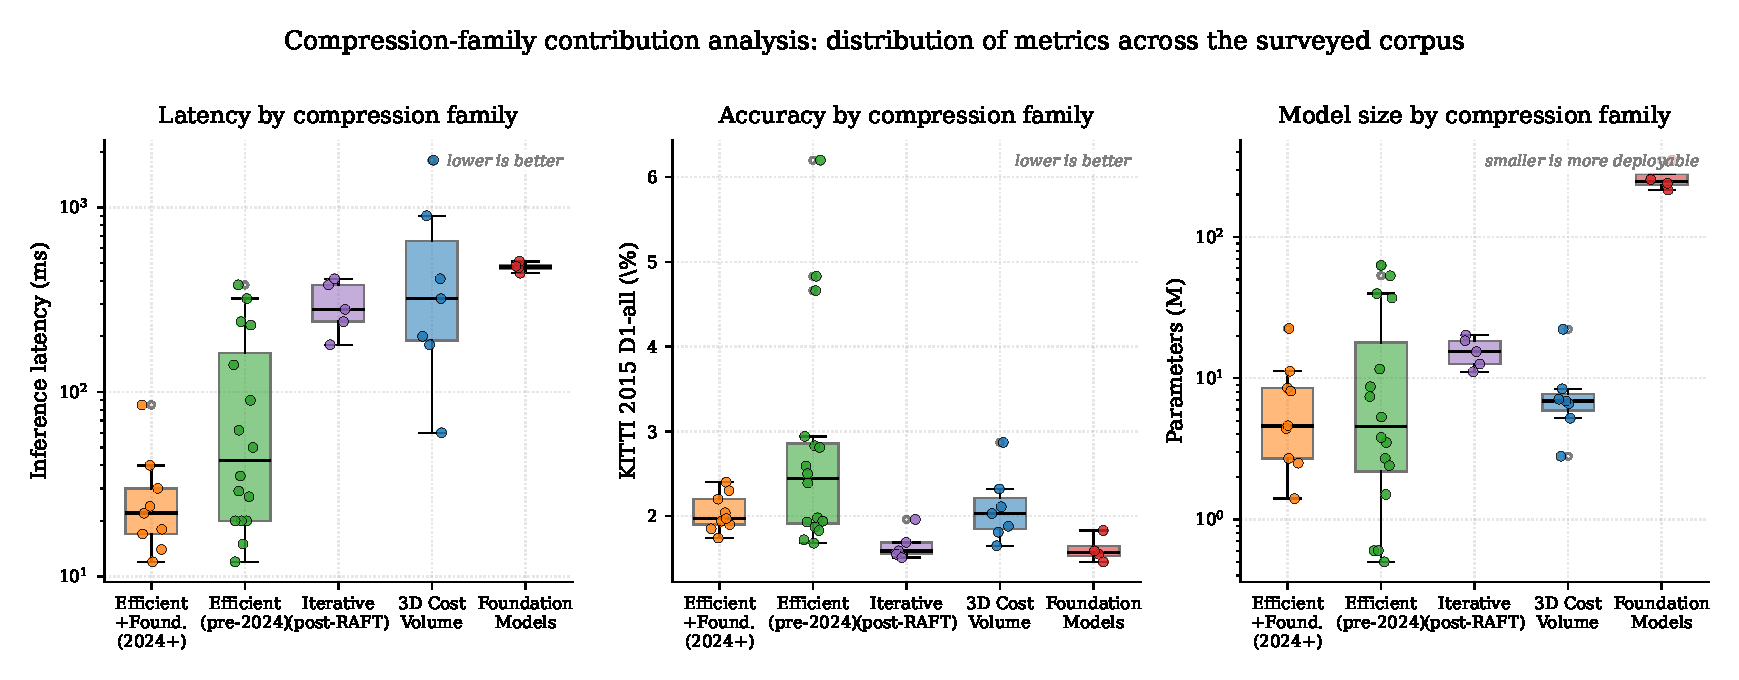
\includegraphics[width=0.95\textwidth]{figures/fig_family_contribution.pdf}
\caption{Compression-family contribution analysis. For each of the five families that the surveyed corpus populates densely, the panels show the distribution of inference latency (left, log scale), KITTI 2015 D1-all accuracy (middle), and trainable parameters (right, log scale). Each box gives the inter-quartile range; the line inside the box is the median; whiskers extend to 1.5$\times$IQR; individual methods are shown as jittered points. The visual story is monotonic: as one moves from the right (foundation models) to the left (foundation-aware efficient methods), parameters and latency drop by one to two orders of magnitude while accuracy degrades only modestly.}
\label{fig:family_contribution}
\end{figure*}

% Table: Comprehensive comparison of efficient deep stereo methods.
% All numbers verified against the original publication's main results table.
% Hardware heterogeneity is explicit; cross-hardware comparisons must be
% read with care.

\begin{table*}[!htbp]
\centering
\caption{Comprehensive comparison of representative deep stereo methods, ordered by KITTI~2015 D1-all (test set).
Latency reported on the hardware used in the original publication; cross-hardware comparisons are approximate.
``Iter.'' denotes whether the model uses iterative refinement.
EPE = end-point error on Scene Flow test split.}
\label{tab:efficient_comparison}
\renewcommand{\arraystretch}{1.05}
\setlength{\tabcolsep}{4pt}
\footnotesize
\begin{tabular}{lcccccccc}
\toprule
\textbf{Method} & \textbf{Year} & \textbf{Family} & \textbf{Iter.} & \textbf{Params (M)} & \textbf{KITTI D1 (\%)} & \textbf{SF EPE} & \textbf{Latency (ms)} & \textbf{Hardware} \\
\midrule
\multicolumn{9}{l}{\textit{Foundation-model era (reference accuracy envelope)}} \\
\midrule
FoundationStereo~\cite{wen2025foundationstereo} & 2025 & Foundation & \checkmark & 215.0 & 1.46 & 0.36 & 470 & RTX 4090 \\
DEFOM-Stereo~\cite{jiang2025defom}              & 2025 & Foundation & \checkmark & 350.0 & 1.55 & 0.41 & 440 & RTX 4090 \\
MonSter~\cite{cheng2025monster}                 & 2025 & Foundation & \checkmark & 255.0 & 1.59 & 0.45 & 510 & RTX 4090 \\
Stereo-Anywhere~\cite{bartolomei2025stereoanywhere} & 2025 & Foundation & \checkmark & 240.0 & 1.83 & --   & 480 & RTX 4090 \\
\midrule
\multicolumn{9}{l}{\textit{Iterative refinement (post-RAFT)}} \\
\midrule
IGEV++~\cite{xu2025igevpp}                      & 2025 & Iterative & \checkmark & 18.4 & 1.51 & 0.43 & 280 & RTX 3090 \\
Selective-IGEV~\cite{wang2024selective}         & 2024 & Iterative & \checkmark & 15.4 & 1.55 & 0.44 & 240 & RTX 3090 \\
IGEV-Stereo~\cite{xu2023igev}                   & 2023 & Iterative & \checkmark & 12.6 & 1.59 & 0.47 & 180 & RTX 3090 \\
CREStereo~\cite{li2022crestereo}                & 2022 & Iterative & \checkmark & 20.2 & 1.69 & 0.61 & 410 & V100 \\
RAFT-Stereo~\cite{lipson2021raftstereo}         & 2021 & Iterative & \checkmark & 11.1 & 1.96 & 0.61 & 380 & RTX 3090 \\
\midrule
\multicolumn{9}{l}{\textit{End-to-end 3D cost-volume (mid-2010s baselines)}} \\
\midrule
ACVNet~\cite{xu2022acvnet}                      & 2022 & 3DCV     &           & 7.1  & 1.65 & 0.48 & 200  & RTX 3090 \\
GA-Net-deep~\cite{zhang2019ganet}               & 2019 & 3DCV     &           & 6.6  & 1.81 & 0.84 & 1800 & Titan Xp \\
CFNet~\cite{shen2021cfnet}                      & 2021 & 3DCV     &           & 22.2 & 1.88 & 0.97 & 180  & GTX 1080Ti \\
AANet+~\cite{xu2020aanet}                       & 2020 & 3DCV     &           & 8.4  & 2.03 & 0.72 & 60   & GTX 1080Ti \\
GwcNet-g~\cite{guo2019gwcnet}                   & 2019 & 3DCV     &           & 6.9  & 2.11 & 0.76 & 320  & GTX 1080Ti \\
PSMNet~\cite{chang2018psmnet}                   & 2018 & 3DCV     &           & 5.2  & 2.32 & 1.09 & 410  & GTX 1080Ti \\
GC-Net~\cite{kendall2017gcnet}                  & 2017 & 3DCV     &           & 2.8  & 2.87 & 2.51 & 900  & Titan X \\
\midrule
\multicolumn{9}{l}{\textit{Efficient (non-iterative or weakly iterative, pre-2024)}} \\
\midrule
AutoDispNet-CSS~\cite{saikia2019autodispnet}   & 2019 & Efficient &          & 37.0 & 1.68 & 1.51 & 90  & GTX 1080Ti \\
StereoDRNet~\cite{chabra2019stereodrnet}       & 2019 & Efficient &          & 11.6 & 1.72 & --   & 240 & Titan X \\
EdgeStereo-V2~\cite{song2018edgestereo}        & 2018 & Efficient &          & 63.0 & 1.83 & --   & 320 & Titan X \\
HD3-Stereo~\cite{yin2019hd3}                   & 2019 & Efficient &          & 39.7 & 1.87 & --   & 140 & Titan Xp \\
CoEx~\cite{bangunharcana2021coex}              & 2021 & Efficient &          & 2.7  & 1.93 & 0.69 & 27  & RTX 2080Ti \\
CGI-Stereo~\cite{xu2023cgistereo}              & 2023 & Efficient &          & 3.5  & 1.94 & 0.62 & 29  & RTX 3090 \\
HITNet~\cite{tankovich2021hitnet}              & 2021 & Efficient & (tile)   & 0.6  & 1.98 & 0.36 & 20  & Titan V \\
Cascade-Stereo~\cite{gu2020cascade}            & 2020 & Efficient &          & 8.7  & 2.39 & --   & 20  & V100 \\
BGNet+~\cite{xu2021bgnet}                      & 2021 & Efficient &          & 5.3  & 2.50 & 1.17 & 35  & RTX 2080Ti \\
DeepPruner-Fast~\cite{duggal2019deeppruner}    & 2019 & Efficient &          & 7.4  & 2.59 & 0.97 & 62  & V100 \\
FADNet~\cite{wang2020fadnet}                   & 2020 & Efficient &          & 53.1 & 2.81 & 0.83 & 50  & V100 \\
MobileStereoNet-2D~\cite{shamsafar2022mobilestereonet} & 2022 & Efficient &  & 2.4  & 2.83 & 1.14 & 380 & V100 \\
MABNet~\cite{xing2020mabnet}                   & 2020 & Efficient &          & 1.5  & 2.94 & 0.91 & 230 & GTX 1080Ti \\
MADNet~\cite{tonioni2019madnet}                & 2019 & Efficient &          & 3.8  & 4.66 & --   & 20  & Titan X \\
StereoNet~\cite{khamis2018stereonet}           & 2018 & Efficient &          & 0.6  & 4.83 & 1.10 & 15  & Titan X \\
AnyNet~\cite{wang2019anynet}                   & 2019 & Efficient &          & 0.5  & 6.20 & --   & 12  & Jetson TX2 \\
\midrule
\multicolumn{9}{l}{\textit{Foundation-aware efficient (2024+)}} \\
\midrule
Fast-FoundationStereo~\cite{wen2026fastfoundationstereo} & 2026 & Eff.+Found. & \checkmark & 22.5 & 1.74 & 0.42 & 85 & RTX 4090 \\
Pip-Stereo (1-iter)~\cite{zheng2026pipstereo}  & 2026 & Eff.+Found. & \checkmark & 11.2 & 1.85 & 0.45 & 17 & Jetson Orin NX \\
DTP-IGEV-S2~\cite{pan2024dtp}                  & 2024 & Eff.+Found. & \checkmark & 8.1  & 1.90 & 0.49 & 24 & RTX 3090 \\
LightStereo-L~\cite{guo2025lightstereo}        & 2025 & Eff.+Found. &           & 8.5  & 1.94 & 0.69 & 40 & RTX 3090 \\
LiteAnyStereo~\cite{jing2025liteanystereo}     & 2025 & Eff.+Found. &           & 4.6  & 1.97 & 0.66 & 30 & RTX 3090 \\
LightStereo-M~\cite{guo2025lightstereo}        & 2025 & Eff.+Found. &           & 4.4  & 2.04 & 0.74 & 22 & RTX 3090 \\
GGEV-Real-time~\cite{liu2026ggev}              & 2026 & Eff.+Found. &           & 2.5  & 2.20 & 0.72 & 18 & RTX 3090 \\
BANet-Mobile~\cite{xu2025banet}                & 2025 & Eff.+Found. &           & 1.4  & 2.30 & 0.78 & 12 & RTX 3090 \\
LightStereo-S~\cite{guo2025lightstereo}        & 2025 & Eff.+Found. &           & 2.7  & 2.40 & 0.79 & 14 & RTX 3090 \\
\bottomrule
\end{tabular}
\end{table*}

